\documentclass{article}
\usepackage[italian]{babel}
\usepackage[T1]{fontenc}
\usepackage[utf8]{inputenc}
\usepackage{pgfplots}
\pgfplotsset{compat=1.12}
\usepgfplotslibrary{fillbetween}
\usetikzlibrary{patterns, quotes, angles}
\usepackage{amsmath}
\usepackage{textcomp}
\usepackage{booktabs}
\usepackage{amsfonts}
\usepackage{mathtools}
\usepackage[hidelinks]{hyperref}
\graphicspath{ {./img/} }




\title{Complex Numbers}
\author{Lorenzo Bonanni}
\date{October 2021}

\usetikzlibrary{math}
\tikzmath{
  function sinc(\x) {
    if  abs(\x) < .001 then { % (|x| < .001) ~ (x = 0)
      return 1;
    } else {
      return sin(\x r)/\x;
    };
  };
}


\begin{document}
    \clearpage

    \begin{titlepage}
       \centering
       \vspace*{\fill}
       {\scshape\LARGE Università degli Studi di Verona \par}
       \vspace{1.5cm}
       \line(1,0){145} \\
       {\huge\bfseries Elaborazione Segnali e Immagini\par}
       \line(1,0){145} \\
       \vspace{0.5cm}
       {\scshape\Large Appunti del corso\par}
       \vspace{2cm}
       {\Large\itshape Lorenzo Bonanni \par}
       \vspace{1cm}

       \vspace{5cm}
       \vspace*{\fill}
       % Bottom of the page
       {\large \today\par}
    \end{titlepage}
    \thispagestyle{empty}

    \tableofcontents

    \section{Fondamenti}
    \subsection{Numeri Complessi}
    I numeri complessi sono numeri che vengono espressi nella seguente forma\\ $c=Re+jIm$
    
    \noindent
    \begin{minipage}{.5\textwidth}
        Essi sono rappresentati sul piano complesso mostrando sull'asse delle X la componente reale e sull'asse delle Y la componente Immaginaria
    \end{minipage}
    \hspace{0.5cm}
    \begin{minipage}{.4\textwidth}
        \begin{tikzpicture}[scale=2.3,cap=round,>=latex]
            % draw the coordinates
            \draw[->] (0cm,0cm) -- (1.2cm,0cm) node[right,fill=white] {$Re$};
            \draw[->] (0cm,0cm) -- (0cm,1.2cm) node[above,fill=white] {$Im$};
        
            \draw
                (0.7,0.7) coordinate (a) node[right,fill=white] {$c$}
                -- (0,0) coordinate (o)
                -- (1,0) coordinate (c) 
                pic["$\Theta$", color=blue, draw=blue, -, angle eccentricity=1.5, angle radius=1cm]
                {angle=c--o--a};
            
            \draw[dotted, thick, color=blue] (0.7,0.7) -- (0.7,0);
            
            \draw[dotted, thick, color=blue] (0.7,0.7) -- (0,0.7);
                
        \end{tikzpicture}
    \end{minipage}
    
    \noindent
    Un numero complesso può essere definito
    \begin{itemize}
        \item \textbf{Forma Vettoriale}: $c=Re+jIm$
        \item \textbf{Forma Polare}: $c=|c|(cos(\theta)+jsin(\theta))$
    \end{itemize}

    \noindent
    Quest'ultima forma può essere riscritta seguendo la formula di Eulero come $\color{red}|c|e^{j\theta}$ dove $|c|$ è chiamato modulo e rappresenta la lunghezza del vettore mentre $\theta$ è chiamato fase.\\
    
    \noindent
    L'evoluzione è il Fasore ovvero una funzione $\mathbb{R}\rightarrow\mathbb{C}$ fatta nel seguente modo:\\$|c|e^{j\theta(t)}$ in questa funzione $\theta$ non è più fisso ma è una funzione del tempo.\\
    Questa funzione permette di modellare la posizione di un punto
    che ruota attorno all’origine con raggio determinato $|c|$ e e velocità angolare costante $\theta(t)$.\\
    
    \noindent
    Così facendo disegno dei cerchi nel piano complesso, la funzione $\theta$ può essere utile riscriverla come:
    $\Theta(t)=\frac{2\pi}{T_0}t+\phi$ \\dove $2\pi$ rappresenta una rotazione attorno al cerchio unitario, $T_0$ rappresenta il tempo necessario ad effettuare tale rotazione e $\phi$ è la fase iniziale
    
    \subsection{Somma Vettoriale}
    la somma di due vettori $\bar{u}$, $\bar{v}$ è un vettore $\bar{w}$ calcolabile geometricamente
    \begin{itemize}
        \begin{minipage}{.4\textwidth}
            \item regola parallelogramma
        \end{minipage}
        \begin{minipage}{.4\textwidth}
            \begin{tikzpicture}[]
                % draw the coordinates
                \draw[->, thick] (0cm,0cm) -- (1.2cm,0cm);
                \draw[->, thick] (0cm,0cm) -- (0cm,1.2cm);
            
                \draw[->, color=red] (0cm,0cm) -- node [midway,above,align=center] {\tiny$\bar{u}$} (0.5cm,0.7cm);
                \draw[->, color=red] (0cm,0cm) -- node [midway,below,align=center] {\tiny$\bar{v}$} (1cm,0.5cm);
                
                \draw[->, color=blue, thick] (0cm,0cm) -- node [midway,above,align=center] {\tiny$\bar{w}$} (1.5cm,1.2cm);
                
                \draw[-, color=red, dashed] (0.5cm,0.7cm) -- (1.5cm,1.2cm);
                \draw[-, color=red, dashed] (1cm,0.5cm) -- (1.5cm,1.2cm);
                
            \end{tikzpicture}
        \end{minipage}
        
        \begin{minipage}{.4\textwidth}
            \item regola punta coda
        \end{minipage}
        \begin{minipage}{.4\textwidth}
            \begin{tikzpicture}[]
                % draw the coordinates
                \draw[->, thick] (0cm,0cm) -- (1.2cm,0cm);
                \draw[->, thick] (0cm,0cm) -- (0cm,1.2cm);
            
                \draw[->, color=red] (0cm,0cm) -- node [midway,above,align=center] {\tiny$\bar{u}$} (0.5cm,0.7cm);
                \draw[->, color=red] (0.5cm,0.7cm) -- node [midway,above,align=center] {\tiny$\bar{v}$} (1.5cm,1.2cm);
                
                \draw[->, color=blue, thick] (0cm,0cm) -- node [midway,below,align=center] {\tiny$\bar{w}$} (1.5cm,1.2cm);
                
            \end{tikzpicture}
        \end{minipage}
    \end{itemize}
    
    \noindent
    \begin{center}
        $\bar{w} = \bar{u}+\bar{v}$
    \end{center}
\newpage
\subsection{Serie di Fourier}
    mi fa capire il contenuto frequienziale di un segnale di periodo T ed è espressa ne seguente modo:
    \begin{align*}
        f(t)=\sum_{n=-\infty}^{+\infty} c_n\cdot e^{\frac{j2\pi n}{T}t}
    \end{align*}
    \begin{center}
        dove $e^{\frac{j2\pi n}{T}t}$ è un fasore con modulo 1
    \end{center}
    
\subsection{Funzioni Pari e Dispari}
    \subsubsection{Funzioni Pari}
        Una funzione $f:\mathbb{R}\rightarrow\mathbb{R}$ è pari sse: $f(t)=f(-t)$\\
        Ovvero ho una simmetria rispetto all'asse delle $y$
        \begin{center}
            \begin{tikzpicture}[domain = -7:7, samples = 1000, scale=0.8]
                % grid
                \draw[very thin, color = gray, step=1] (-8,-2.2) grid(8,2.2);
            
                % Axes:
            	\draw [->, thick] (-8,0) -- (8,0);
            	\draw [->, thick] (0,-2.2) -- (0,2.2);
        
                \draw[very thick, color = green!55!gray] plot[id=c] function{cos(2*x)};
            \end{tikzpicture}
        \end{center}

    \subsubsection{Funzioni Dispari}
        Una funzione $f:\mathbb{R}\rightarrow\mathbb{R}$ è dispari sse: $f(t)=-f(-t)$\\
        Ovvero la funzione è speculare rispetto all'asse delle $x$ cioè dato un punto $x$ e un punto $-x$ essi avranno coordinate sull'asse dell $y$ opposte ((-1, 1), (0.5, -0.5)...)
        \begin{center}
            \begin{tikzpicture}[domain = -7:7, samples = 1000, scale=0.8]
                % grid
                \draw[very thin, color = gray, step=1] (-8,-2.2) grid(8,2.2);
            
                % Axes:
            	\draw [->, thick] (-8,0) -- (8,0);
            	\draw [->, thick] (0,-2.2) -- (0,2.2);
        
                \draw[very thick, color = blue] plot[id=c] function{sin(2*x)};
            \end{tikzpicture}
        \end{center}
    \newpage
    
    \subsection{Segnali Periodici}
        Un segnale $f$ è periodico di periodo T o T-periodo se:\\
        \begin{center}
            $\exists T_0\in R^+:f(t+T_0)=f(t),\quad \forall t\in D_1$
        \end{center}
        e $T_0$ è il minor numero per cui la condizione di ripetizione si verifica\\
        
        \noindent
        Dato un periodo $T_0$ si usa indicare con $\mu_0$ la "frequenza fondamentale"\\ $\mu_0=1/T_0$ misurata in Hz
    \subsection{Segnali Periodici-Trigonometrici}
    Fissato $T_0>0$ i segnali trigonometrici di minimo periodo $T_0$ sono:\\
    \begin{center}
        $f(t)=cos2\pi\mu_0t \qquad\qquad f(t)=sin2\pi\mu_0t$
    \end{center}
    dove $\mu$ è una frequenza, $\mu_0=\frac{1}{T_0}$ \textit{frequenza fondamentale}\\
    
    \noindent
    La formula $2\pi\mu_0$ può anche essere scritta come $\frac{2\pi}{T_0}$
    
    \subsection{Operazioni Fondamentali}
    Dati due segnali $f,g$ arbitrari (monodimensionali)
    
    \begin{itemize}
        \item \textbf{SOMMA} $h(t)=f(t)+g(t)\quad\forall t\in D_1$\\
        Funzioni che non si sovrappongono\\
        %f(t)
        \begin{minipage}{.15\textwidth}
            \begin{tikzpicture}[domain = -1.5:0, samples = 1000, scale=0.5]
            
                % Axes:
            	\draw [->, thick] (-2,0) -- (2,0);
            	\draw [->, thick] (0,-1.8) -- (0,1.8) node[right,fill=white] {$f(t)$};
        
                \draw[very thick, color = green!55!gray] plot function{cos(2*x)};
            \end{tikzpicture}
        \end{minipage}
        \hspace{0.2cm}
        \begin{minipage}{.05\textwidth}
            \textbf{+}
        \end{minipage}
        \begin{minipage}{.15\textwidth}
            \begin{tikzpicture}[domain = 0:1.5, samples = 1000, scale=0.5]
            
                % Axes:
            	\draw [->, thick] (-2,0) -- (2,0);
            	\draw [->, thick] (0,-1.8) -- (0,1.8) node[right,fill=white] {$g(t)$};
        
                \draw[very thick, color = blue] plot function{cos(2*x)};
            \end{tikzpicture}
        \end{minipage}
        \hspace{0.2cm}
        \begin{minipage}{.05\textwidth}
            \textbf{+}
        \end{minipage}
        \begin{minipage}{.15\textwidth}
            \begin{tikzpicture}[domain = -1.5:1.5, samples = 1000, scale=0.5]
            
                % Axes:
            	\draw [->, thick] (-2,0) -- (2,0);
            	\draw [->, thick] (0,-1.8) -- (0,1.8) node[right,fill=white] {$f(t)+g(t)$};
        
                \draw[very thick] plot function{cos(2*x)};
            \end{tikzpicture}
        \end{minipage}
        
        Funzioni che si sovrappongono\\
        %f(t)
        \begin{minipage}{.15\textwidth}
            \begin{tikzpicture}[domain = -1.5:0, samples = 1000, scale=0.5]
            
                % Axes:
            	\draw [->, thick] (-2,0) -- (2,0);
            	\draw [->, thick] (0,-1.8) -- (0,1.8) node[right,fill=white] {$f(t)$};
        
                \draw[very thick, color = green!55!gray] (-1, 0) -- (0, 1.2);
                \draw[very thick, color = green!55!gray] (1, 0) -- (0, 1.2);
            \end{tikzpicture}
        \end{minipage}
        \hspace{0.2cm}
        \begin{minipage}{.05\textwidth}
            \textbf{+}
        \end{minipage}
        \begin{minipage}{.15\textwidth}
            \begin{tikzpicture}[domain = 0:1.5, samples = 1000, scale=0.5]
            
                % Axes:
            	\draw [->, thick] (-2,0) -- (2,0);
            	\draw [->, thick] (0,-1.8) -- (0,1.8) node[right,fill=white] {$g(t)$};
        
                \draw[very thick, color = blue] (0, 0) -- (1, -1.2);
                \draw[very thick, color = blue] (1, -1.2) -- (2, 0);
            \end{tikzpicture}
        \end{minipage}
        \hspace{0.2cm}
        \begin{minipage}{.05\textwidth}
            \textbf{+}
        \end{minipage}
        \begin{minipage}{.15\textwidth}
            \begin{tikzpicture}[domain = -1.5:1.5, samples = 1000, scale=0.5]
            
                % Axes:
            	\draw [->, thick] (-2,0) -- (2,0);
            	\draw [->, thick] (0,-1.8) -- (0,1.8) node[right,fill=white] {$f(t)+g(t)$};
        
                \draw[very thick] (-1, 0) -- (0, 1.2);
                \draw[very thick] (0, 1.2) -- (1, -1.2);
                \draw[very thick] (1, -1.2) -- (2, 0);
            \end{tikzpicture}
        \end{minipage}
        \item \textbf{PRODOTTO} $h(t)=f(t)\cdot g(t)\quad\forall t\in D_1$
        \item \textbf{AMPLIFICAZIONE} $h(t)=\lambda f(t)\quad\forall t\in D_1$
        \item \textbf{SHIFT(o TRASLAZIONE)} $\forall f(t):D_1\in\mathbb{R}, \quad \tau\in\mathbb{R}^+$\\
            \begin{tikzpicture}[scale=0.5]
                % Axes:
            	\draw [->, thick] (-2,0) -- (5,0);
            	\draw [->, thick] (0,-0.5) -- (0,2.5) node[right,fill=white] {$f(t-\tau)$};
        
                \draw[dashed, thick] (-1, 0) -- (-1, 2) -- (1, 2) -- (1, 0);
                \draw[->, color=red] (1, 1) -- node [midway,above right,align=center] {$+\tau$} (4.5, 1);
                \draw[thick] (2.5, 0) -- (2.5, 2) -- (4.5, 2) -- (4.5, 0);
            \end{tikzpicture}
        \item \textbf{RESCALING(o RISCALATURA)} $\forall f(t): D_1\in\mathbb{R},\quad \omega\neq 0$\\
        ritardo o accelero \textbf{linearmente} il segnale di un fattore $\omega$\\
        \begin{center}
            \begin{minipage}{.15\textwidth}
                \begin{center}
                    \textbf{f(t)}
                \end{center}
                \begin{tikzpicture}[scale=0.5]
                    % Axes:
                	\draw [->, thick] (-2,0) -- (3,0);
                	\draw [->, thick] (0,-0.5) -- (0,3.5);
            
                    \draw[thick] (-1, 0) node [below, align=center] {\small$-c$} -- (-1, 2) 
                                         -- (1, 2) 
                                         -- (1, 0) node [below, align=center] {\small$c$};
                \end{tikzpicture}
            \end{minipage}
            \hspace{1cm}
            \begin{minipage}{.5\textwidth}
                \begin{minipage}{.5\textwidth}
                    \begin{center}
                        Ritardo
                        $f(\omega t), \quad 0<\omega<1$
                    \end{center}
                    \begin{tikzpicture}[scale=0.5]
                        % Axes:
                    	\draw [->, thick] (-2.5,0) -- (3,0);
                    	\draw [->, thick] (0,-0.5) -- (0,3.5);
                
                        \draw[thick] (-2, 0) node [below, align=center] {\small$-c/\omega$} -- (-2, 2) 
                                             -- (2, 2) 
                                             -- (2, 0) node [below, align=center] {\small$c/\omega$};
                    \end{tikzpicture}
                \end{minipage}
        
                \begin{minipage}{.5\textwidth}
                    \begin{center}
                        Accellero
                        $f(\omega t), \quad \omega>1$
                    \end{center}
                    \begin{tikzpicture}[scale=0.5]
                        % Axes:
                    	\draw [->, thick] (-2,0) -- (3,0);
                    	\draw [->, thick] (0,-0.5) -- (0,3.5);
                
                        \draw[thick] (-0.5, 0) node [below] {\tiny$-c/\omega$} -- (-0.5, 2) 
                                             -- (0.5, 2) 
                                             -- (0.5, 0) node [below] {\tiny$c/\omega$};
                    \end{tikzpicture}
                \end{minipage}
            \end{minipage}
        \end{center}
        \item \textbf{CROSS-CORRELAZIONE}
        Dati $f_1(\tau), f_2(\tau)$ segnali continui, $\tau\in\mathbb{R}$, il segnale di cross-correlazione è
        \begin{align*}
            f_1\otimes f_2(t)=\int_{-\infty}^{\infty} f^{*}_{1}(\tau)f_{2}(\tau-t)d\tau
        \end{align*}
            \begin{itemize}
                \item $f^{*}_{1}(\tau)$ è un complesso coniugato
                \item con t=0 si ha l'integrale di cross-correlazione
                \item Il segnale di cross-correlazione è definito se l'integrale converge(se ho segnali ne' di energia ne' di potenza non ho convergenza)
                \item il valore di cross correlazione è massimo quando i due segnali coincidono
                \item il valore massimo  di cross correlazione mi indica di quanto devo shiftare un segnale per massimizzare la similarità tra i due segnali
                \item la cross-correlazione è robusta al rumore
            \end{itemize}
            Per capire meglio la cross correlazione vedere il seguente animazione\\ \url{https://gifer.com/en/2xBt}
        \newpage
        \noindent
        \item \textbf{CROSS-CORRELAZIONE NORMALIZZATA}\\
        Serve per trattare segnali con range di valori diversi
        \begin{align*}
            f_1\bar{\otimes}f_2(t)=\frac{\int_{-\infty}^{\infty} f^{*}_{1}(\tau)f_{2}(\tau-t)d\tau}{\sqrt{E_{f1}E_{f2}}}
        \end{align*}
        dove $E_f$ indica l'energia del segnale $f$
            \begin{itemize}
                \item $f_1\bar{\otimes}f_2(t)\in[-1,1]$
                \item Nel caso di segnali discreti l'integrale viene sostituito da una sommatoria
                \begin{align*}
                    x_1\otimes x_2(n)=\sum_{k=-\infty}^{\infty} x^{*}_{1}(k)x_{2}(k-n)\quad k\in\mathbb{Z}
                \end{align*}
                \item Nel caso 2D $x_1$ e $x_2$ possono essere pensate come immagini infinite
                \begin{align*}
                    x_1\otimes x_2(m,n)=\sum_{u=-\infty}^{\infty}\sum_{v=-\infty}^{\infty} x_{1}(u,v)x_{2}(u-m,v-m)\quad u,v,m,n\in\mathbb{Z}
                \end{align*}
            \end{itemize}
        \item \textbf{CONVOLUZIONE}\\
        Dati $f_1(t), f_2(t)$ segnali continui di variabile reale, l'integrale di convoluzione è
        \begin{align*}
            f_1\ast f_2(t)=\int_{-\infty}^{\infty}f_1(\tau)f_2(t-\tau)d\tau
        \end{align*}
        Simile alla cross-correlazione solo che invece di $\tau-t$ metto $-(\tau-t)=(t-\tau)$\\
        Nel caso di segnali discreti la formula diventa:
        \begin{align*}
            x_1\ast x_2(n)=\sum_{k=-\infty}^{\infty}x_1(n)x_2(n-k)\quad k\in\mathbb{Z}
        \end{align*}
    \end{itemize}
    \subsection{Segnali Continui di uso Comune}
    \subsubsection{Funzione box}
    \textbf{Funzione box} (su x continuo e reale):\\
    $\Pi(x)=\begin{cases}
        1, \quad -0.5\leq x\leq 0.5\\
        0, \quad altrimenti
    \end{cases}$\\
    
    \noindent
    \textbf{Funzione box generica:}\\
    \begin{minipage}{.5\textwidth}
        $A\Pi(x/b)\quad x\in[-b/2,b/2]$\\
    \end{minipage}
    \begin{minipage}{.15\textwidth}
        \begin{tikzpicture}[scale=0.5]
            % Axes:
        	\draw [->, thick] (-2,0) -- (3,0);
        	\draw [->, thick] (0,-0.5) -- (0,3.5) node[right] {$A\Pi(x/b)$};
    
            \draw[thick] (-1, 0) node [below, align=center] {\small$-b/2$} -- (-1, 2) 
                                 -- node [midway,above right,align=center] {\small$A$} (1, 2) 
                                 -- (1, 0) node [below, align=center] {\small$b/2$};
        \end{tikzpicture}
    \end{minipage}
    \subsubsection{Impulso di Dirac}
    \textbf{Impulso Unitario}\\
    L'impulso unitario è una funzione definita nel seguente modo:
    \begin{align*}
        \delta(x)=\lim_{b\to 0} \frac{1}{b}\Pi(x/b)\quad colvincolo \int_{-\infty}^{\infty} \delta(x)dx=1
    \end{align*}\\
    
    \noindent
    Percui:\\[0.2cm]
    \begin{minipage}{.5\textwidth}
        $\delta(x)=\begin{cases}
        \infty\quad se \, x=0\\
        0 \quad se \, x\neq 0\\
    \end{cases}$
    \end{minipage}
    \begin{minipage}{.5\textwidth}
        \begin{align*}
            \int_{-\infty}^{\infty} \delta(x)dx=1
        \end{align*}
    \end{minipage}
    \vspace{0.3cm}
    
    \noindent
    \textbf{Impulso Traslato}\\
    \begin{align*}
        \delta(x-x_0)=\lim_{b\to 0} \frac{1}{b}\Pi(\frac{x-x_0}{b})\quad col vincolo \int_{-\infty}^{\infty} \delta(x)dx=1
    \end{align*}
    \vspace{0.3cm}
    
    \noindent
    Proprietà dell’impulso:
    \begin{enumerate}
        \item $\delta(x-x_0)=0\quad\forall x\neq x_0$
        \item Proprietà di Setacciamento\\
        \begin{equation}
            \int_{-\infty}^{\infty} f(x)\delta(x-x_0)dt = f(x_0)
        \end{equation}
        \item $\delta(x-x_0) = \delta(x_0-x)\quad\forall x\in\mathbb{R}$
        \item $\delta(ax)=\frac{1}{|a|}\delta(x)\forall x\in\mathbb{R}$, fissato $a\in\mathbb{R}-{0}$
    \end{enumerate}
    
    \noindent
    \subsubsection{Funzione sinc}
    
    \begin{minipage}{.5\textwidth}
        Caratteristiche:
        \begin{itemize}
            \item Intersezione asse x in 1,2,3...
            \item $\lim_{t\to 0} sinc(t)=0$
        \end{itemize}
        Questa funzione è cluciale per l'analisi tempo/frequenza e inoltre ha uno strettissimo legame con la funzione box
        \begin{align*}
            sinc(t) = \frac{sin(\pi t)}{\pi t}
        \end{align*}
    \end{minipage}
    \begin{minipage}{.4\textwidth}
        \begin{center}
            \begin{tikzpicture}[scale=0.6]
                    \begin{axis}
                        \addplot [domain = -720:720, samples = 200, color=red, thick]{sin(x)/ (x*pi/180) };
                    \end{axis}
            \end{tikzpicture}
        \end{center}
    \end{minipage}
    
    \noindent
    \subsubsection{Funzione triangolo}
    
    \begin{minipage}{.4\textwidth}
        \begin{center}
           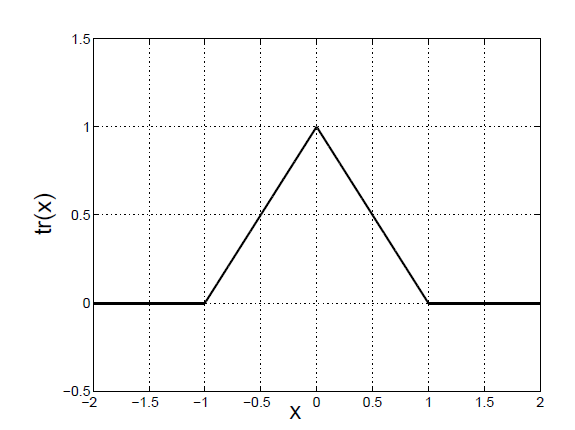
\includegraphics[scale=0.2]{triangle.png}
        \end{center}
    \end{minipage}
    \begin{minipage}{.5\textwidth}
        Importante nell’analisi spettrale e per le operazioni di convoluzione
        \begin{align*}
            \Lambda(x)=\begin{cases}
                1-|x|, \quad |x|<1\\
                0\quad altrimenti
            \end{cases}
        \end{align*}
    \end{minipage}
    
    \noindent
    \subsubsection{Funzione Segno}
    
    \begin{minipage}{.5\textwidth}
        Ribalta segnali sopra/sotto l’asse x
        \begin{align*}
            \Lambda(x)=\begin{cases}
                -1, \quad x<0\\
                +1\quad x>0\\
                0\quad x=0
            \end{cases}
        \end{align*}
    \end{minipage}
    \begin{minipage}{.4\textwidth}
        \begin{center}
           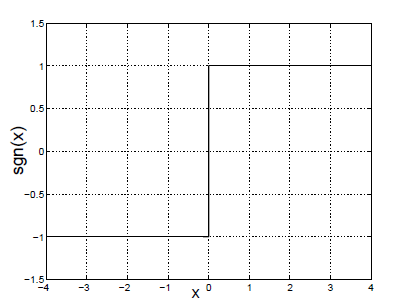
\includegraphics[scale=0.3]{sign.png}
        \end{center}
    \end{minipage}
    
     \noindent
    \subsubsection{Funzione gradino}
    
    \begin{minipage}{.4\textwidth}
        \begin{center}
           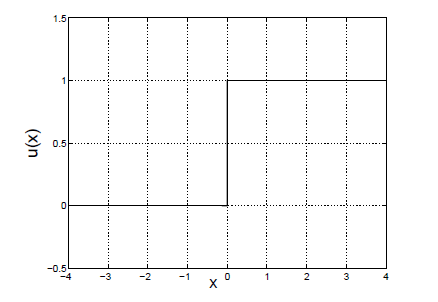
\includegraphics[scale=0.3]{gradino.png}
        \end{center}
    \end{minipage}
    \begin{minipage}{.5\textwidth}
        rappresenta un segnale che si attiva a partire da un tempo specificato e rimane attivo indefinitamente
        \begin{align*}
            \Lambda(x)=\begin{cases}
                0, \quad x<0\\
                1\quad x\geq0
            \end{cases}
        \end{align*}
    \end{minipage}
    
    \noindent
    \subsubsection{Treno di Impulsi}
    
    \begin{minipage}{.5\textwidth}
        Il treno di impulsi $S_{\Delta T}(x)$ è a somma di un numero infinito di impulsi periodici discreti distanziati di una quantità $\Delta T$
        \begin{align*}
            S_{\Delta T}(x)=\sum_{-\infty}^{\infty}    \delta(x-n\Delta T) \quad n\in\mathbb{Z}\\
            \delta(x)=\begin{cases}
            1\quad se \, x=0\\
            0 \quad se \, x\neq 0\\
            \end{cases}
        \end{align*}
    \end{minipage}
    \begin{minipage}{.4\textwidth}
        \begin{center}
            \begin{tikzpicture}[scale=0.6]
                \draw [->, thick] (-3.5,0) -- (3.5,0);
                \foreach \x in {-3,...,0,...,3}{
                    \draw [->] (\x, 0) node [below, scale=0.5] {$\x\Delta T$} -- (\x, 3);
                }
            \end{tikzpicture}
        \end{center}
    \end{minipage}
    \subsection{Energia di un Segnale}
    \begin{minipage}{.4\textwidth}
        Un segnale si dice ad energia finita (o di energia) se l’integrale che ne rappresenta l’energia converge ed è diverso da 0.\\
        Tale condizione è sufficiente all'esistenza della trasformata di Fourier, eccezion fatta per le funzioni trigonometriche le quali non sono di energia ma hanno la Trasformata di Fourier.
        L'energia si misura di Joule.
    \end{minipage}
    \hspace{0.2cm}
    \begin{minipage}{.5\textwidth}
        \begin{align*}
                E_f=\begin{cases}
                     \int_{-\infty}^{\infty} f^2(t)dt \qquad se f\in\mathbb{R}\\
                     \int_{-\infty}^{\infty} |f(t)|^2dt \quad con |f(t)|^2=f^*(t)f(t), f \in\mathbb{C}
                \end{cases}
        \end{align*}
    \end{minipage}
    
    \subsection{Potenza media di un segnale}
    Un segnale si dice a potenza finita (o di potenza) se l'integrale che ne rappresenta la potenza converge ed è diverso da 0. La potenza si misura in Watt.\\
    Il valore $\frac{1}{T}$ serve per rendere comparabili fra loro segnali di estensione diversa.
    Un segnale non può essere sia di energia che di potenza perchè per un segnale ad energia finita la potenza tende a 0.\\
    Infine esistono segnali che non sono né di energia ne di potenza (ad esempio $e^{at}$)
    \begin{align*}
        P_f=\begin{cases}
           \lim_{T\to\infty}\frac{1}{T}\int_{-\frac{T}{2}}^{+\frac{T}{2}} f^2(t)dt \qquad se f\in\mathbb{R}\\
           \lim_{T\to\infty}\frac{1}{T}\int_{-\frac{T}{2}}^{+\frac{T}{2}} |f(t)|^2dt \quad con |f(t)|^2=f^*(t)f(t), f \in\mathbb{C}
        \end{cases}
    \end{align*}
    
\end{document}
